\section{Results}
	\label{sec:results}
	
	\begin{figure}[t]
		\centering
		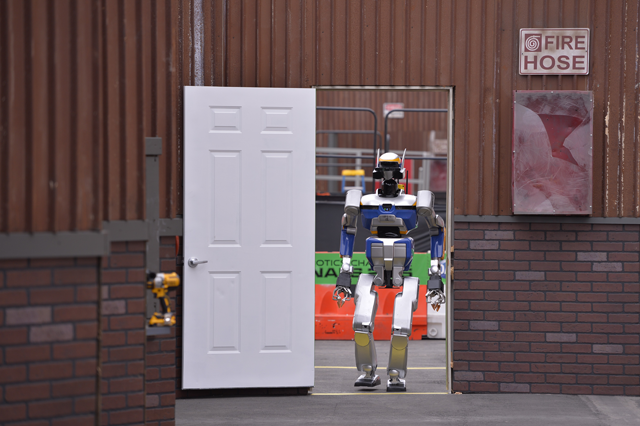
\includegraphics[height = 5.5cm]{img/door-drc}
		\caption{Door Task at the DARPA Robotics Challenge~\cite{DARPA}.}
		\label{fig:door-drc}
	\end{figure}
	
	\begin{figure}[t]
		\centering
		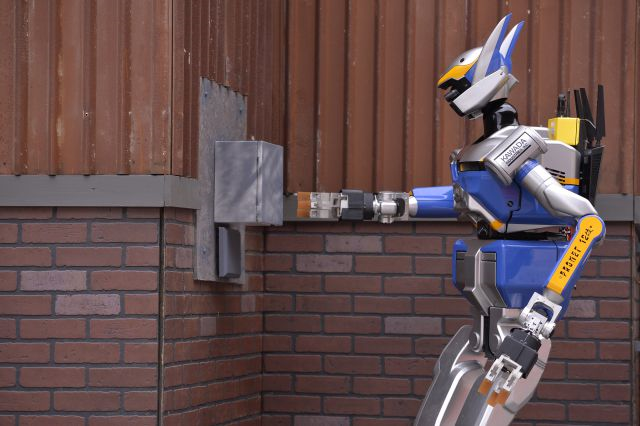
\includegraphics[height = 5.5cm]{img/button-drc}
		\caption{Button Task at the rehersal of the DARPA Robotics Challenge~\cite{DARPA}.}
		\label{fig:button-drc}
	\end{figure}
	
	With respect to the plug task, during the DRC Finals we were able to complete the task
	and get the point	within 16 minutes and 34 seconds, mainly because we were supervising
	every motion of the robot in order to prevent any collision with the environment, and
	also due to blackouts.
	Some snapshots taken during the task at the DRC Finals are shown in
	\figurename~\ref{fig:plug-drc}, together with the description of the current process
	in accordance with the explanation given before.
	
	\begin{figure}[t]
		\centering
		\subfloat[Adjust manipulation marker]
			{\label{fig:Plug_30_24_60} 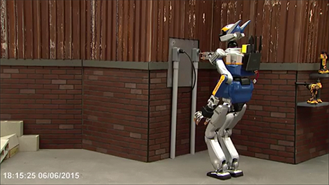
\includegraphics[height = 2cm]{img/Plug_30_24_60}}
		\subfloat[Adjust point cloud offset]
			{\label{fig:Plug_32_24_23} 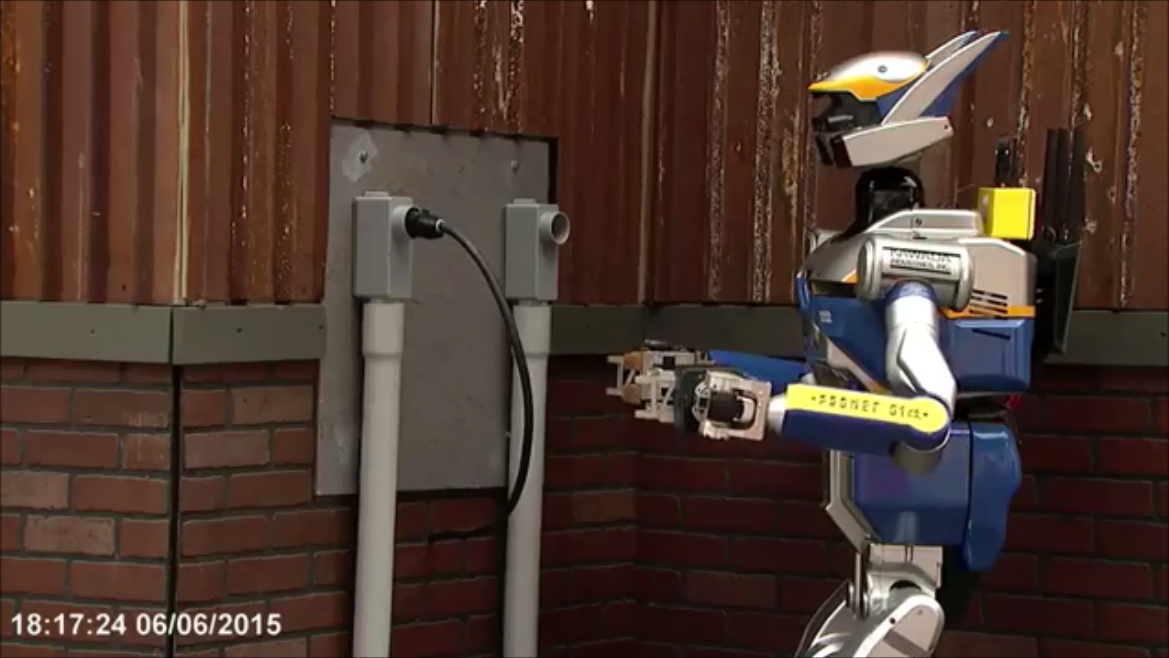
\includegraphics[height = 2cm]{img/Plug_32_24_23}}
		\\
		%
		\subfloat[Adjust hand for pre-grasping]
			{\label{fig:Plug_34_33_87} 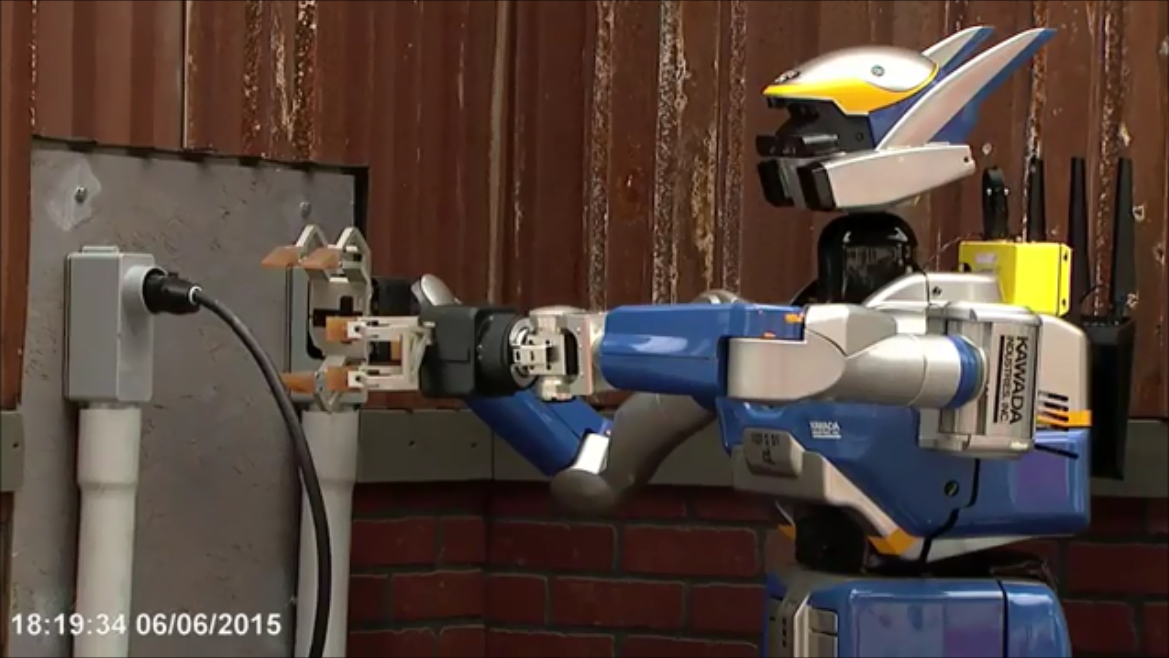
\includegraphics[height = 2cm]{img/Plug_34_33_87}}
		\subfloat[Align hand to grasp]
			{\label{fig:Plug_37_23_37} 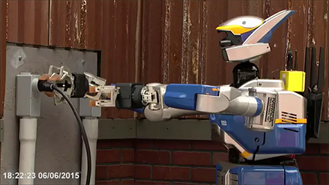
\includegraphics[height = 2cm]{img/Plug_37_23_37}}
		\\
		%
		\subfloat[Pull out the plug]
			{\label{fig:Plug_38_13_00} 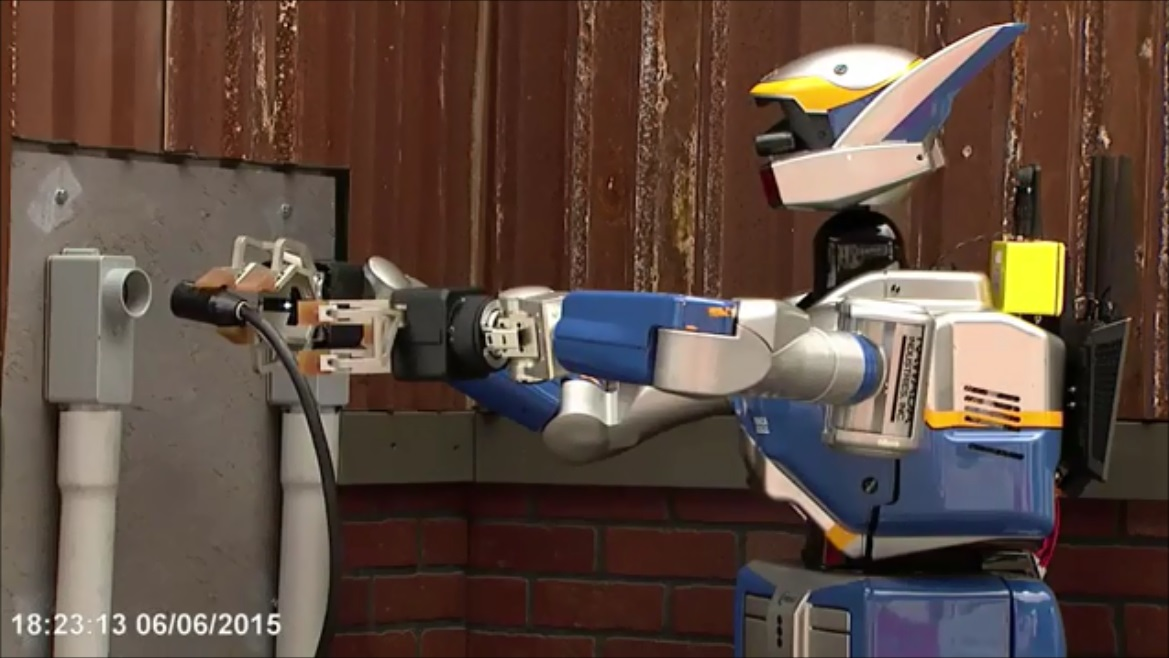
\includegraphics[height = 2cm]{img/Plug_38_13_00}}
		\subfloat[Adjust manipulation marker]
			{\label{fig:Plug_39_03_07} 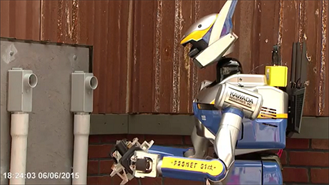
\includegraphics[height = 2cm]{img/Plug_39_03_07}}
		\\
		%
		\subfloat[Adjust hand for pre-insertion]
			{\label{fig:Plug_43_42_13} 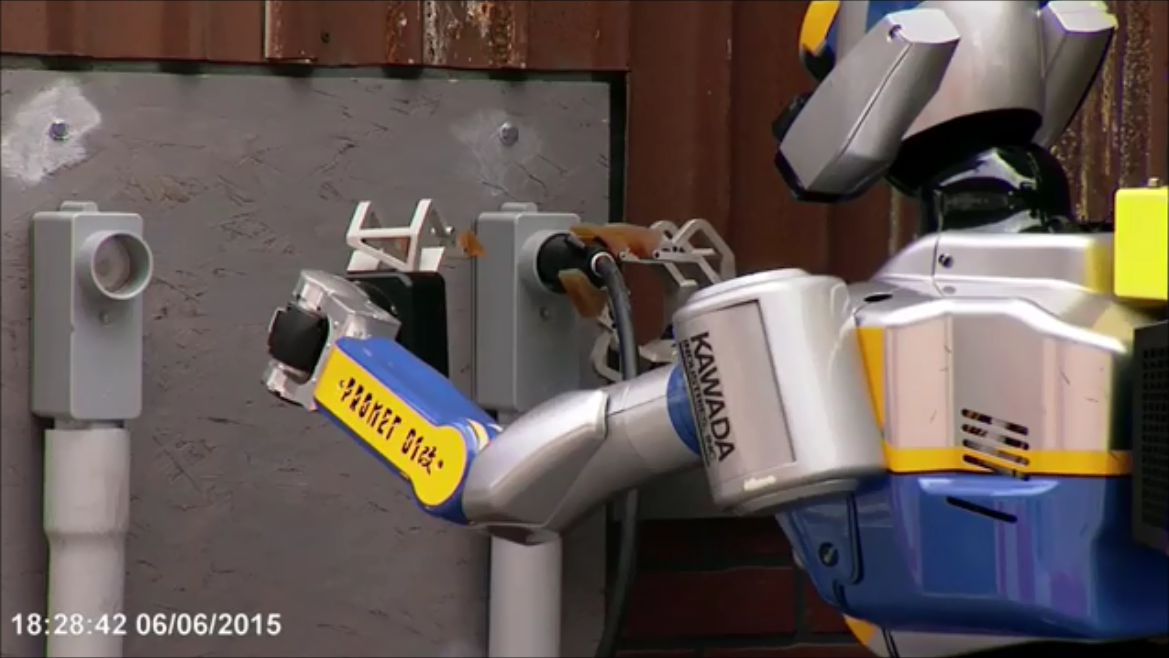
\includegraphics[height = 2cm]{img/Plug_43_42_13}}
		\subfloat[Plug is inserted]
			{\label{fig:Plug_44_51_93} 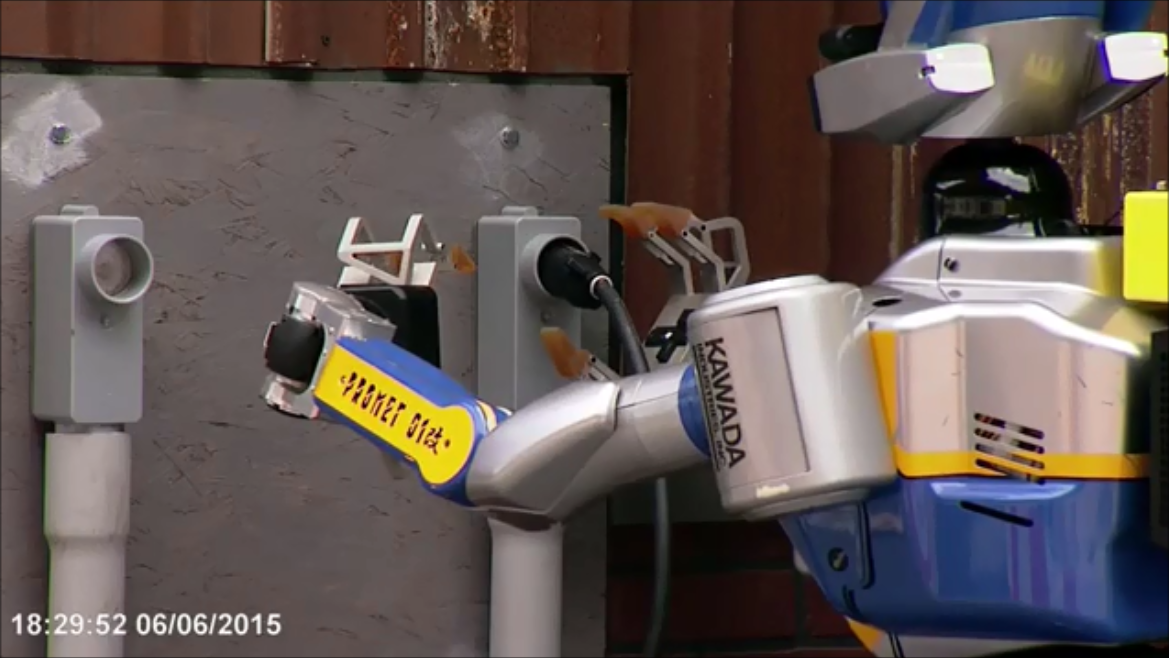
\includegraphics[height = 2cm]{img/Plug_44_51_93}}
		%
		\caption{Plug Task at the second day of the DARPA Robotics Challenge~\cite{DARPA}}
		\label{fig:plug-drc}
	\end{figure}